\chapter{explosions one to four}
\lhead[tempest]{}
\label{sec:if}
\lstset{style=6502Style}

It is almost impossible to notice when playing the game, but the explosion of enemies
in \textit{Tempest} is an animated sequence. It happens so quickly, in just a few frames,
that the effect is almost subliminal: you can somehow detect that the explosion is animated if you look straight at it,
but you cannot actually see it.

Since we have the luxury of slowing things down to a page-turning crawl let's look at the four frames
of the explosion sequence one by one. We will also get to notice the particular economy with which it is
achieved. 

We'll start with an explosion in its infancy. On the left we show the code that defines how the explosion
is drawn. The first three lines contain parameters used by the main drawing routine \icode{SPOK16}. With
a scaling factor of just \icode{1} given by \icode{CM}, the explosion starts small:
\begin{figure}[H]
      \centering
      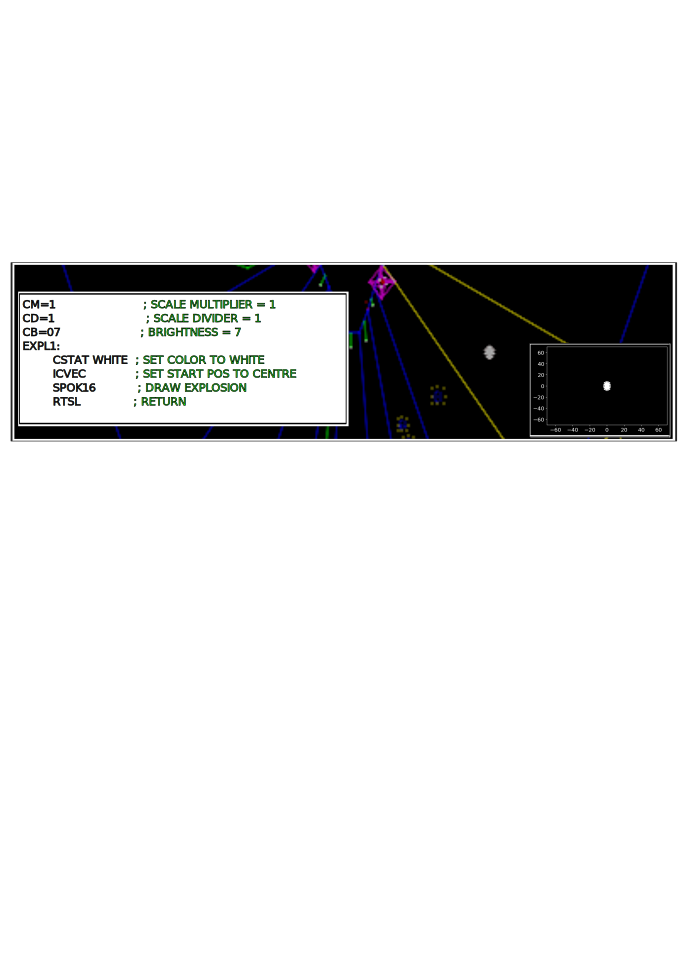
\includegraphics[width=13.4cm]{src/explosions/expl1-comic.png}%
\end{figure}
\vspace{-0.2cm}

When we move on to the second frame of the explosion we start to see some progress, but may be surprised
that the code for \icode{EXPL2} is identical to \icode{EXPL1}. We have to look closely to observe the
only actual difference, the scaling factor of \icode{CM} is now set to \icode{2}. This has the
apparently magical effect of scaling up the explosion by a second order of magnitude.
\begin{figure}[H]
      \centering
      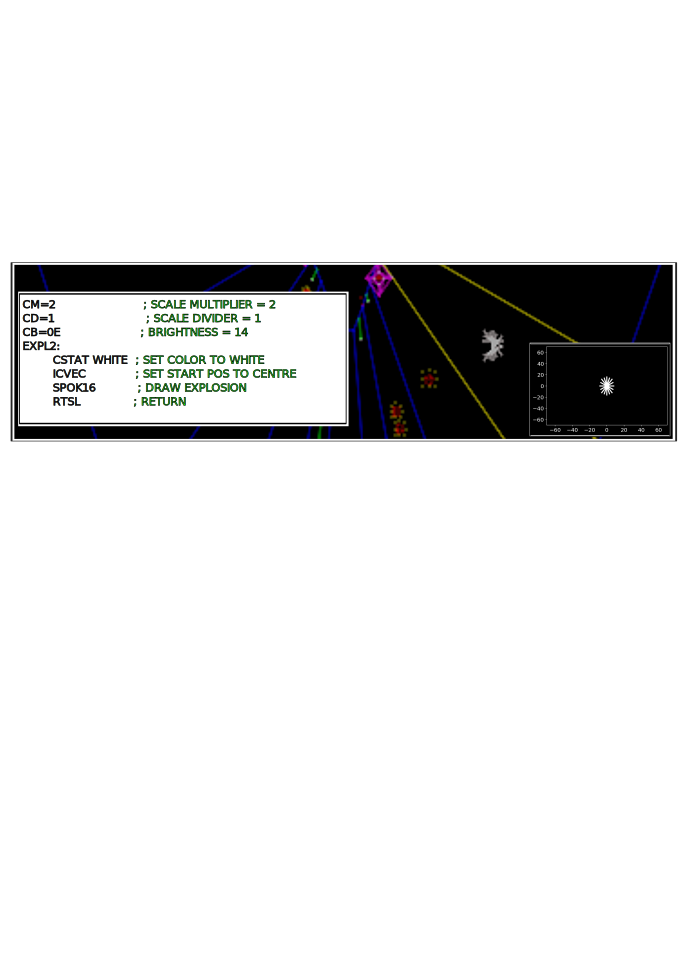
\includegraphics[width=13.4cm]{src/explosions/expl2-comic.png}%
\end{figure}
\vspace{-0.2cm}

To understand this magic we first have to take a look at the \icode{SPOK16} routine being used to
do the actual drawing.

\begin{lstlisting}
.MACRO SPOK16           ; INPUT: CM=SCALE MULTIPLIER
                        ;        CB=INTENSITY
                        ;        CD=SCALE DIVIDER
    ICVEC               ; SET STARTING POINT TO CENTRE
    SCVEC 7,3           ; DRAW A LINE FROM 0,0 TO 7,3.
    SCVEC -7,-3,CB      ; DRAW A LINE FROM 7,3 to -7,-3.
    SCVEC -6,-6         ; DRAW A LINE FROM -7,-3 TO -6,-6. 
    SCVEC 6,6,CB        ; DRAW A LINE FROM 
    SCVEC 3,7           ; DRAW A LINE FROM 
    SCVEC -3,-7,CB      ; DRAW A LINE FROM 
    SCVEC 0,-8          ; DRAW A LINE FROM 
    SCVEC 0,8,CB        ; DRAW A LINE FROM 
    SCVEC -3,7          ; DRAW A LINE FROM 
    SCVEC 3,-7,CB       ; DRAW A LINE FROM 
    SCVEC 6,-6          ; DRAW A LINE FROM 
    SCVEC -6,6,CB       ; DRAW A LINE FROM 
    SCVEC -7,3          ; DRAW A LINE FROM 
    SCVEC 7,-3,CB       ; DRAW A LINE FROM 
    SCVEC 8,0           ; DRAW A LINE FROM 
    SCVEC -8,0,CB       ; DRAW A LINE FROM 
    SCVEC 0,0           ; DRAW A LINE FROM 
.ENDM                    
\end{lstlisting}

At first the relevant magic is not apparent at all. \icode{SPOK16} draws our 16-spoked star-shaped
explosion but uses the same co-ordinates each time. Where does the scaling happen? The answer
to this lies under the hood in \icode{SCVEC}, which is yet another \textit{macro} that takes
the hardcoded co-ordinates in icode{SPOK16} as parameters:

\begin{lstlisting}
.MACRO SCVEC ...A,...B         ; A = X CO-ORD, B = Y CO-ORD
    CVEC ...A*CM/CD,...B*CM/CD ; SCALE UP CO-ORDS USING CM AND CD.
.ENDM
\end{lstlisting}

As you can see above it is in \icode{SCVEC} that the scaling actually happens. The mysterious constant
\icode{CM} we saw in our first two diagrams finally comes in to play and is used to multiply the X and
Y co-ordinates to achieve a scaling effect. For the indefatigably curious, I have given the contents
of the \icode{CVEC} macro below. This is where the hard yards are run to turn the co-ordinates into
a line. Notice that it has to keep track of the position of the previous line in \icode{OLX} and \icode{OLZ}:

\begin{lstlisting}
.MACRO CVEC NEWX,NEWZ,BRIT
  ...XN = NEWX-...OLX
  ...ZN = NEWZ-...OLZ
  ...BR=BRIT
  CS=1
  VCTR ...XN*CS,...ZN*CS,...BR
  ...OLX = NEWX
  ...OLZ = NEWZ
.ENDM
\end{lstlisting}

With the mystery of how our scaling works pretty much solved we can take a look what happens in the next
frame, with our scale factor set to \icode{4}.

\begin{figure}[H]
      \centering
      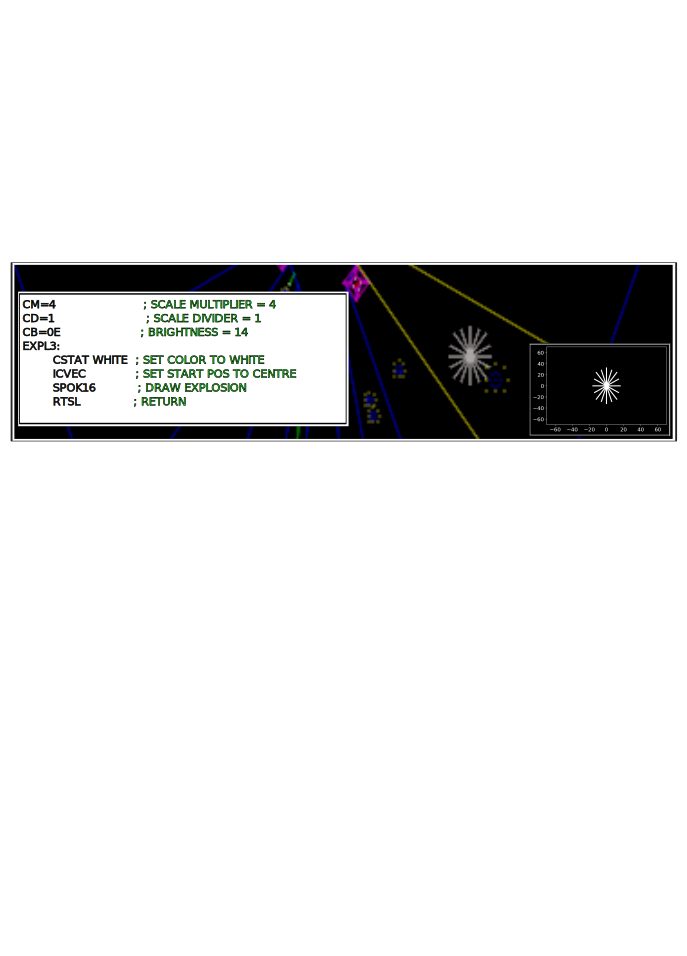
\includegraphics[width=13.4cm]{src/explosions/expl3-comic.png}%
\end{figure}
\vspace{-0.2cm}
And in the final frame of the explosion, \icode{EXPL4}, where the factor is set to \icode{8}, the enemy's
destruction reaches its fullest extent.

\begin{figure}[H]
      \centering
      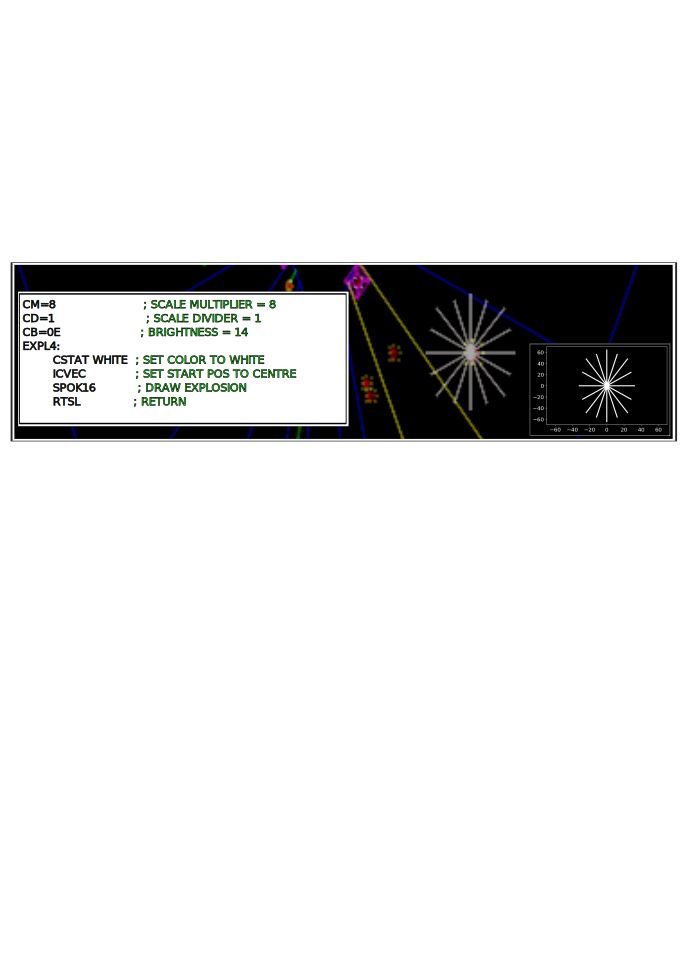
\includegraphics[width=13.4cm]{src/explosions/expl4-comic.png}%
\end{figure}
\vspace{-0.2cm}

\iffalse
\begin{lstlisting}
        .SBTTL  PLAY-PROCESS EXPLOSIONS
PROEXP:
        LDA EXPCOU
        IFNE                    ;ANY BANGS?
        LDA I,0                 ;YES CLEAR COUNT
        STA EXPCOU
        LDX I,NEXPLO-1
        BEGIN                   ;LOOP FOR ACH EXPLOSION
        LDA X,EXPLOY
        IFNE                    ;ACTIVE BANG?
        LDA X,EXPLOS            ;YES. UPDATE SEQUENCES
        LDY X,EXPLOT
        CLC
        ADC Y,TEXINC
        STA X,EXPLOS
        CMP Y,TEXPDN
        IFCS                    ;EXPLOSION DONE?
        LDA I,0                 ;YES. DEACTIVATE IT
        STA X,EXPLOY
        ELSE
        INC EXPCOU              ;NO. INC COUNTER
        ENDIF
        ENDIF
        DEX
        MIEND
        ENDIF
        RTS
TEXPDN: .BYTE 10,15,20,20,20,10         ;LAST SEQUENCE # TABLE(*4)
TEXINC: .BYTE 3,1,3,3,3,3
\end{lstlisting}

\begin{lstlisting}
        .SBTTL  DISPLAY-EXPLOSIONS

DSPEXP:
        LDY I,EXPCOL
        STY COLOR
        LDX I,NEXPLO-1
        STX INDEX1
        BEGIN                   ;LOOP FOR EACH BANG
        LDX INDEX1
        LDA X,EXPLOY
        IFNE                    ;ACTIVE BANG?
        STA PYL                 ;YES SAVE DEPTH
        LDA X,EXPLOL            ;SET UP GRID LINES
        STA TEMP0
        LDY X,EXPLOT            ;CALC. PICTURE TO USE
        CPY I,1
        IFEQ                    ;CHARGE-PLAYER?
        JSR CHPLKI              ;YES.
        ELSE                    ;NO
        LDA X,EXPLOS
        LSR
        AND I,0FE
        CPY I,2
        IFCS
        LDA I,0                 ;NO SEQUENCE TYPE
        ENDIF
        CLC
        ADC Y,TEXTYP
        LDY TEMP0
        JSR SCAPIC              ;DO EXPLOSION PICTURE
        ENDIF
        ENDIF
        DEC INDEX1
        MIEND
ZQPOKS::        LDA QT4
        IFNE                    ;POKEY DOESN'T STOP
        LDA CURWAV
        CMP I,13.
        IFCS
        STA 1FF                 ;KILL TOP OF STACK
        ENDIF
        ENDIF
        RTS
TEXTYP:                 ;START CODE FOR EACH BANG TYPE
        .BYTE PTEXP1            ;CHARGE CHARGE, CHARGE INVADER
        .BYTE 0         ;CHARGE-PLAYER SEE SPECIAL
        .BYTE PTFUSX+4          ;BUSE EXPL 1
        .BYTE PTFUSX+2          ;FUSE EXPL 2
        .BYTE PTFUSX+0          ;FUSE EXPLOSIN 3
        .BYTE PTSPAR                    ;INVADER - PLAYER COLLISION
\end{lstlisting}
\fi
